\part{数学}

\chapter{数论}

\section{线性筛}
\entrymeta{$O(n)$}
\begin{codeline}
class Sieve {
public:
    int pcnt = 0;
    vector<bool> is_not_prime;
    vector<int> prime, phi, mu;

    /*
     * 筛出1..maxn的素数、phi和mu，清空上次结果
     */
    void calc(int maxn) {
        pcnt = 0;
        prime.clear();
        is_not_prime.assign(maxn + 1, false);
        phi.assign(maxn + 1, 0);
        mu.assign(maxn + 1, 0);
        is_not_prime[0] = true;
        if(maxn >= 1) {
            is_not_prime[1] = true;
            phi[1] = mu[1] = 1;
        }
        for(int i = 2; i <= maxn; i++) {
            if(!is_not_prime[i]) {
                prime.push_back(i);
                pcnt++;
                phi[i] = i - 1;
                mu[i] = -1;
            }
            for(int p : prime) {
                if(p > maxn / i) {
                    break;
                }
                is_not_prime[p * i] = true;
                if(i % p == 0) {
                    phi[p * i] = phi[i] * p;
                    break;
                }
                phi[p * i] = phi[i] * (p - 1);
                mu[p * i] = -mu[i];
            }
        }
    }
};
\end{codeline}
\begin{warnbox}
\texttt{maxn \textgreater{}= 0}；筛表大小按题目上限开。
\end{warnbox}

\section{杜教筛}
\entrymeta{$O(n^{2/3})$}
\begin{center}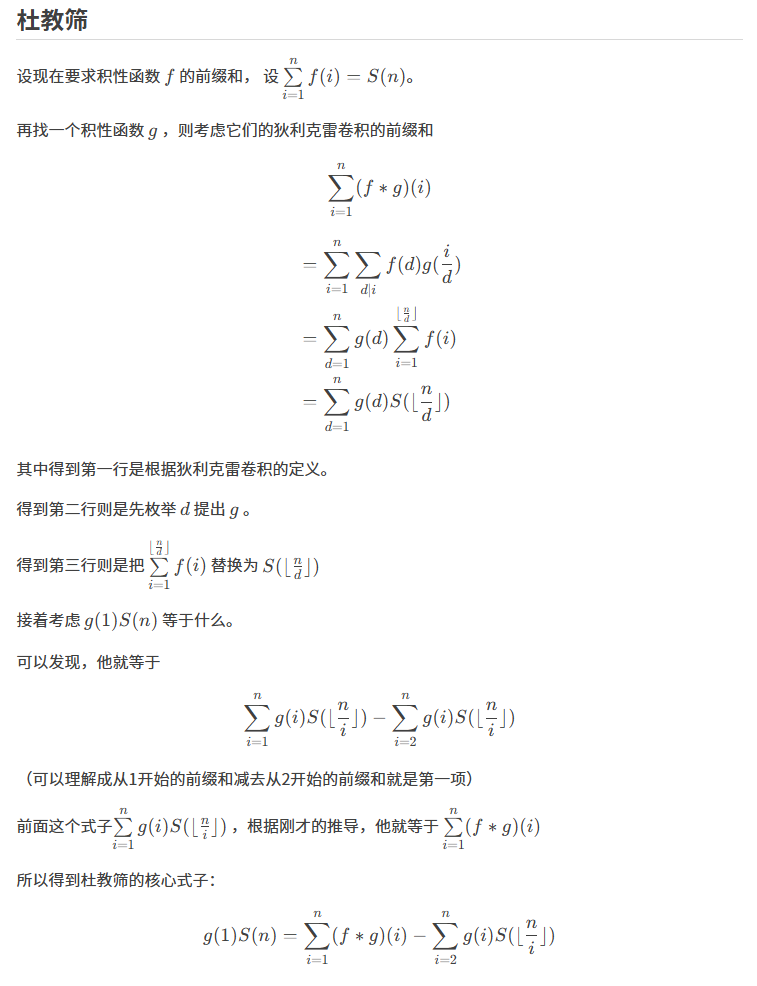
\includegraphics[width=0.78\linewidth]{assets/e041_image-1.png}\end{center}


\begin{codeline}
const int64 N = 1 << 31;

class DusSieve {
    // h = f*g
    // sf = sigma(f)
    // sg = sigma(g)
    // sh = sigma(h)
public:
    const static int64 MAXN = 1 << 21;
    int64 pcnt;

    bool is_not_prime[MAXN];
    int64 prime[MAXN];
    int64 s[MAXN];
    int64 mu[MAXN];
    map<int64, int64> sm;

    int64 f(int64 x) {
        return mu[x];
    }

    int64 g(int64 x) {
        return 1;
    }

    int64 sg(int64 x) {
        return x;
    }

    int64 sh(int64 x) {
        return 1;
    }

    /*
     * 用记忆化整除分块计算f在1..x的前缀和
     */
    int64 sf(int64 x) {
        int64 gs;
        if(x < MAXN) {
            gs = s[x];
        } else if(sm.count(x)) {
            gs = sm[x];
        } else {
            int64 ans = sh(x);
            for(int64 l = 2, r; l <= x; l = r + 1) {
                r = x / (x / l);
\end{codeline}
\vspace{-0.9\baselineskip}
\begin{codeline}[firstnumber=47]
                ans = ans - sf(x / l) * (sg(r) - sg(l - 1));
            }
            gs = sm[x] = ans;
        }
        return gs / g(1);
    }

    /*
     * 线性筛预处理小范围的函数值与前缀和
     */
    void calc(int64 maxn) {}
};

DusSieve sieve;

int main() {
    ios::sync_with_stdio(false);
    cin.tie(nullptr);
    int64 n;
    cin >> n;
    if(n == 1) {
        cout << (0ll) << '\n';
    } else {
        n--;
        sieve.calc(n);
        int64 ans = 0;
        for(int64 l = 1, r; l <= n; l = r + 1) {
            r = n / (n / l);
            ans += (n / l) * (n / l) * (sieve.sf(r) - sieve.sf(l - 1));
        }
        cout << (ans + 2) << '\n';
    }
}
\end{codeline}
\begin{warnbox}
\texttt{calc()} 留空，使用时把线性筛的实现填进来；小范围查表，大范围记忆化整除分块。
\end{warnbox}
\clearpage
\subsection*{延伸阅读}
\begin{center}
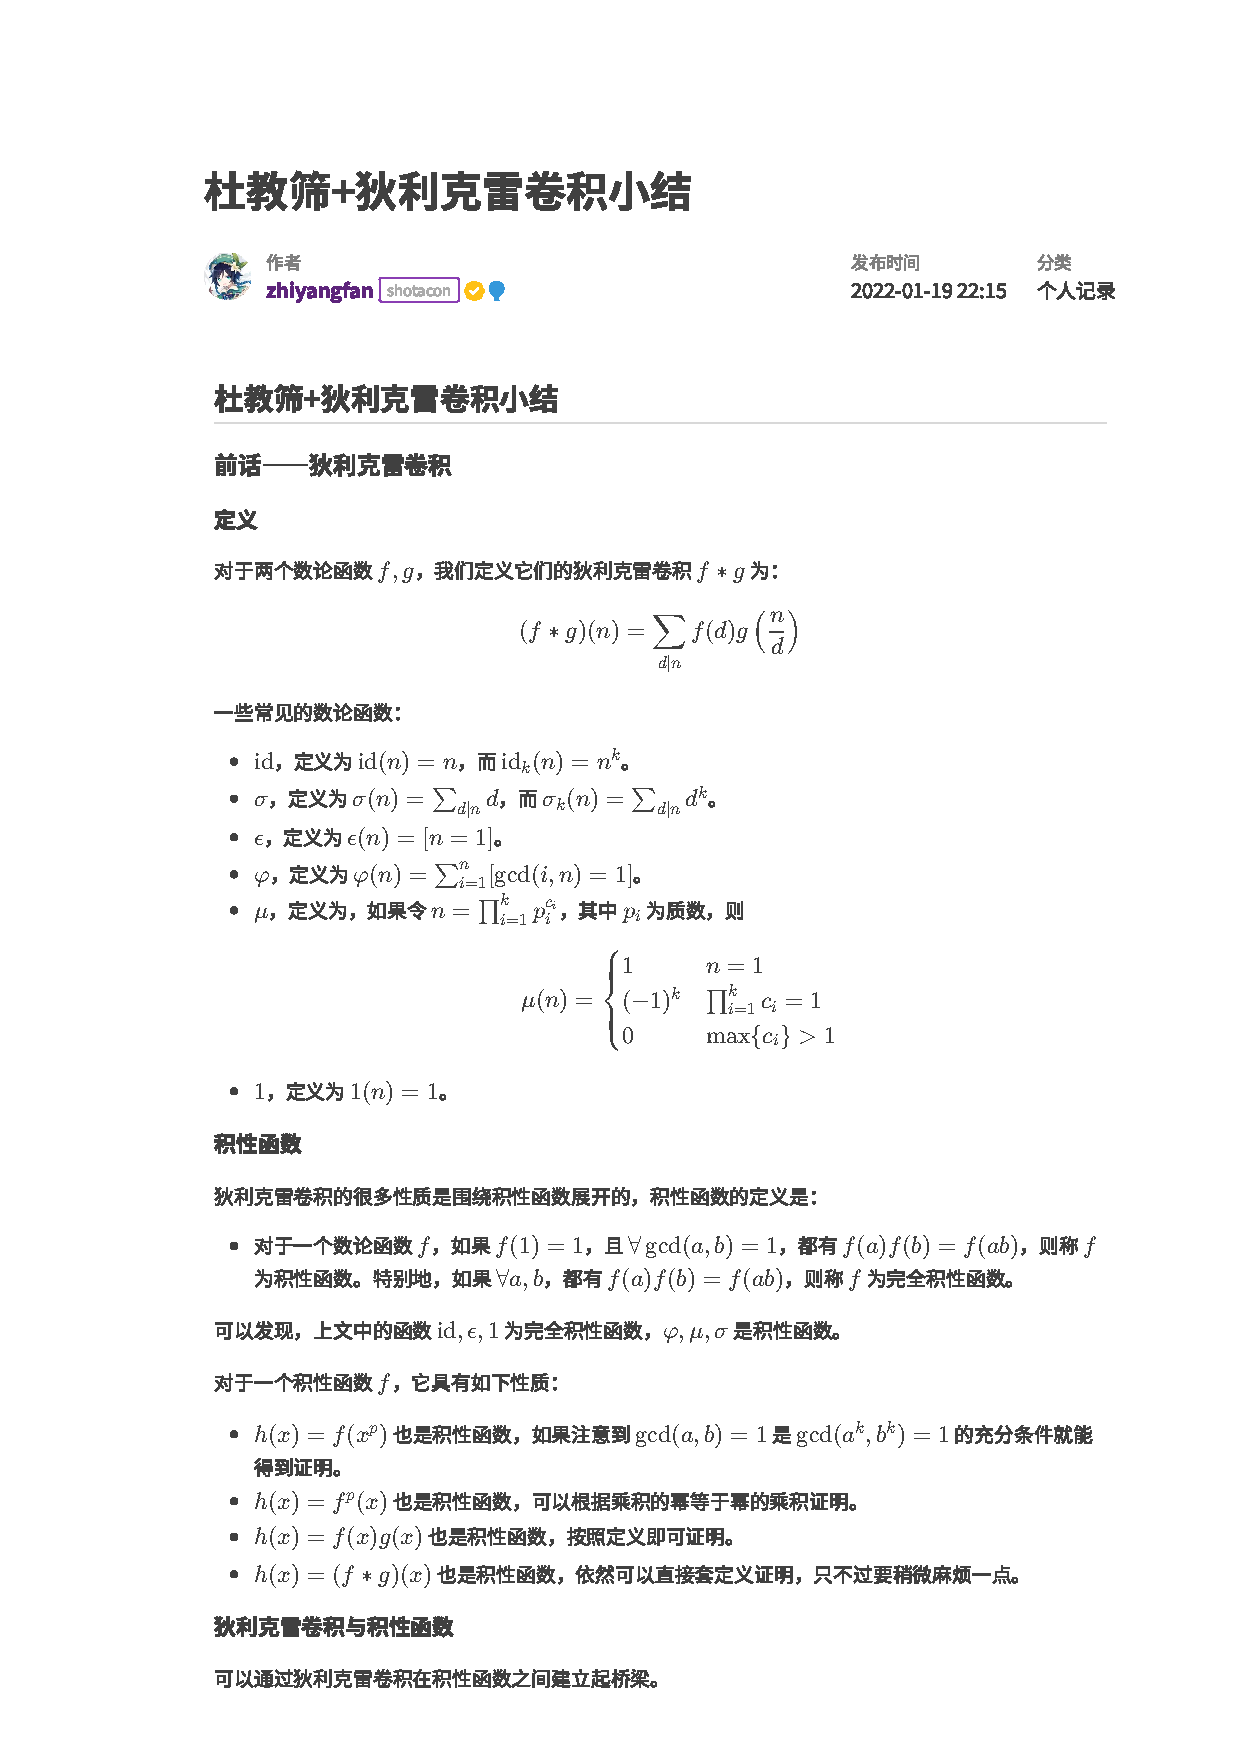
\includegraphics[page=1,width=0.94\linewidth,height=0.90\textheight,keepaspectratio]{assets/pdf/pdf_041.pdf}
\end{center}
\clearpage
\begin{center}
\includegraphics[page=2,width=0.94\linewidth,height=0.90\textheight,keepaspectratio]{assets/pdf/pdf_041.pdf}
\end{center}
\clearpage
\begin{center}
\includegraphics[page=3,width=0.94\linewidth,height=0.90\textheight,keepaspectratio]{assets/pdf/pdf_041.pdf}
\end{center}
\clearpage
\begin{center}
\includegraphics[page=4,width=0.94\linewidth,height=0.90\textheight,keepaspectratio]{assets/pdf/pdf_041.pdf}
\end{center}
\clearpage
\begin{center}
\includegraphics[page=5,width=0.94\linewidth,height=0.90\textheight,keepaspectratio]{assets/pdf/pdf_041.pdf}
\end{center}
\clearpage
\begin{center}
\includegraphics[page=6,width=0.94\linewidth,height=0.90\textheight,keepaspectratio]{assets/pdf/pdf_041.pdf}
\end{center}
\clearpage
\begin{center}
\includegraphics[page=7,width=0.94\linewidth,height=0.90\textheight,keepaspectratio]{assets/pdf/pdf_041.pdf}
\end{center}
\clearpage
\begin{center}
\includegraphics[page=8,width=0.94\linewidth,height=0.90\textheight,keepaspectratio]{assets/pdf/pdf_041.pdf}
\end{center}
\clearpage
\begin{center}
\includegraphics[page=9,width=0.94\linewidth,height=0.90\textheight,keepaspectratio]{assets/pdf/pdf_041.pdf}
\end{center}
\clearpage

\section{迪利克雷前缀和}
\entrymeta{$O(n\log\log n)$}
\subsection{P5495 【模板】Dirichlet 前缀和}\label{p5495-ux6a21ux677fdirichlet-ux524dux7f00ux548c}






\begin{codeline}
const int N = 20000005;
unsigned int seed;
inline unsigned int getnext() {
    seed ^= seed << 13;
    seed ^= seed >> 17;
    seed ^= seed << 5;
    return seed;
}

int n;
bool is_not_prime[N];
unsigned int prime[N];
unsigned int cnt = 0;

class DirichletPrefixSum {
    const static int MAXN = N;

public:
    unsigned int h[MAXN];

    unsigned int g(unsigned int x) {
        return 1u;
    }

    void calc() {
        for(unsigned int i = 0; i < cnt; i++) {
            for(unsigned int j = n / prime[i]; j; j--) {
                for(long long t = prime[i]; j * t <= n; t *= prime[i]) {
                    h[j * t] += h[j] * g(t);
                }
            }
        }
    }
};

DirichletPrefixSum b;

int main() {
    ios::sync_with_stdio(false);
    cin.tie(nullptr);
    cin >> n >> seed;
    for(int i = 1; i <= n; i++) {
        b.h[i] = getnext();
    }

    is_not_prime[0] = true;
\end{codeline}
\vspace{-0.9\baselineskip}
\begin{codeline}[firstnumber=47]
    is_not_prime[1] = true;
    for(unsigned int i = 2; i <= n; i++) {
        if(!is_not_prime[i]) {
            prime[cnt] = i;
            cnt++;
        }
        for(unsigned int j = 0; j < cnt && prime[j] * i <= n; j++) {
            is_not_prime[prime[j] * i] = true;
            if(i % prime[j] == 0) {
                break;
            }
        }
    }

    b.calc();

    unsigned int ans = 0;
    for(unsigned int i = 1; i <= n; i++) {
        ans ^= b.h[i];
    }

    cout << (ans);
}
\end{codeline}
\begin{warnbox}
按质因子降序做后缀和；\texttt{h[j]} 在处理时仍是原数组。
\end{warnbox}

\section{迪利克雷卷积}
\entrymeta{$O(n\log\log n)$}
\subsection{定义}\label{ux5b9aux4e49}

欧拉函数（Euler's totient function），即 \(\varphi(n)\)，表示的是小于等于 \(n\) 和 \(n\) 互质的数的个数。

比如说 \(\varphi(1) = 1\)。

当 \(n\) 是质数的时候，显然有 \(\varphi(n) = n - 1\)。

\subsection{性质}\label{ux6027ux8d28}

\begin{itemize}
\item
  欧拉函数是 \href{./basic.md\#积性函数}{积性函数}。

  即对任意满足 \(\gcd(a, b) = 1\) 的整数 \(a,b\)，有 \(\varphi(ab) = \varphi(a)\varphi(b)\)。

  特别地，当 \(n\) 是奇数时 \(\varphi(2n) = \varphi(n)\)。

  证明参见 \href{./basic.md\#剩余系的复合}{剩余系的复合}。
\item
  \(n = \sum_{d \mid n}{\varphi(d)}\)。

  利用 \href{./mobius.md}{莫比乌斯反演} 相关知识可以得出。

  也可以这样考虑：如果 \(\gcd(k, n) = d\)，那么 \(\gcd(\dfrac{k}{d},\dfrac{n}{d}) = 1, ( k < n )\)。

  如果我们设 \(f(x)\) 表示 \(\gcd(k, n) = x\) 的数的个数，那么 \(n = \sum_{i = 1}^n{f(i)}\)。

  根据上面的证明，我们发现，\(f(x) = \varphi(\dfrac{n}{x})\)，从而 \(n = \sum_{d \mid n}\varphi(\dfrac{n}{d})\)。注意到约数 \(d\) 和 \(\dfrac{n}{d}\) 具有对称性，所以上式化为 \(n = \sum_{d \mid n}\varphi(d)\)。
\item
  若 \(n = p^k\)，其中 \(p\) 是质数，那么 \(\varphi(n) = p^k - p^{k - 1}\)。 （根据定义可知）
\item
  由唯一分解定理，设 \(n = \prod_{i=1}^{s}p_i^{k_i}\)，其中 \(p_i\) 是质数，有 \(\varphi(n) = n \times \prod_{i = 1}^s{\dfrac{p_i - 1}{p_i}}\)。
\item
  引理：设 \(p\) 为任意质数，那么 \(\varphi(p^k)=p^{k-1}\times(p-1)\)。

  证明：显然对于从 1 到 \(p^k\) 的所有数中，除了 \(p^{k-1}\) 个 \(p\) 的倍数以外其它数都与 \(p^k\) 互素，故 \(\varphi(p^k)=p^k-p^{k-1}=p^{k-1}\times(p-1)\)，证毕。

  接下来我们证明 \(\varphi(n) = n \times \prod_{i = 1}^s{\dfrac{p_i - 1}{p_i}}\)。由唯一分解定理与 \(\varphi(x)\) 函数的积性

  \[
  \begin{aligned}
      \varphi(n) &= \prod_{i=1}^{s} \varphi(p_i^{k_i}) \\
      &= \prod_{i=1}^{s} (p_i-1)\times {p_i}^{k_i-1}\\
      &=\prod_{i=1}^{s} {p_i}^{k_i} \times(1 - \frac{1}{p_i})\\
      &=n~ \prod_{i=1}^{s} (1- \frac{1}{p_i})
      &\square
  \end{aligned}
  \]
\item
  对任意不全为 \(0\) 的整数 \(m,n\)，\(\varphi(mn)\varphi(\gcd(m,n))=\varphi(m)\varphi(n)\gcd(m,n)\)。

  可由上一条直接计算得出。
\end{itemize}

\subsection{应用}\label{ux5e94ux7528}

欧拉函数常常用于化简一列最大公约数的和。国内有些文章称它为 \textbf{欧拉反演}{[}\^{}1{]}。

在结论

\[
n=\sum_{d|n}\varphi(d)
\]

中代入 \(n=\gcd(a,b)\)，则有

\[
\gcd(a,b) = \sum_{d|\gcd(a,b)}\varphi(d) = \sum_d [d|a][d|b]\varphi(d),
\]

其中，\([\cdot]\) 称为 \href{https://mathworld.wolfram.com/IversonBracket.html}{Iverson 括号}，只有当命题 \(P\) 为真时 \([P]\) 取值为 \(1\)，否则取 \(0\)。对上式求和，就可以得到

\[
\sum_{i=1}^n\gcd(i,n)=\sum_{d}\sum_{i=1}^n[d|i][d|n]\varphi(d)=\sum_d\left\lfloor\frac{n}{d}\right\rfloor[d|n]\varphi(d)=\sum_{d|n}\left\lfloor\frac{n}{d}\right\rfloor\varphi(d).
\]

这里关键的观察是 \(\sum_{i=1}^n[d|i]=\lfloor\frac{n}{d}\rfloor\)，即在 \(1\) 和 \(n\) 之间能够被 \(d\) 整除的 \(i\) 的个数是 \(\lfloor\frac{n}{d}\rfloor\)。

利用这个式子，就可以遍历约数求和了。需要多组查询的时候，可以预处理欧拉函数的前缀和，利用数论分块查询。

\subsection{欧拉定理}\label{ux6b27ux62c9ux5b9aux7406}

与欧拉函数紧密相关的一个定理就是欧拉定理。其描述如下：

若 \(\gcd(a, m) = 1\)，则 \(a^{\varphi(m)} \equiv 1 \pmod{m}\)。

\subsubsection{扩展欧拉定理}\label{ux6269ux5c55ux6b27ux62c9ux5b9aux7406}

当然也有扩展欧拉定理，用于处理一般的 \(a\) 和 \(m\) 的情形。

\[
a^b\equiv
\begin{cases}
a^{b\bmod\varphi(m)},\,&\gcd(a,\,m)=1\\
a^b,&\gcd(a,\,m)\ne1,\,b<\varphi(m)\\
a^{b\bmod\varphi(m)+\varphi(m)},&\gcd(a,\,m)\ne1,\,b\ge\varphi(m)
\end{cases}
\pmod m
\]

\subsection{P2398 GCD SUM}\label{p2398-gcd-sum}


\begin{codeline}
const int64 N = 100005;
bool is_not_prime[N];
int64 prime[N / 10];
int64 euler[N];

int64 n;
int64 cnt = 0;

int main() {
    ios::sync_with_stdio(false);
    cin.tie(nullptr);
    cin >> n;
    is_not_prime[0] = true;
    is_not_prime[1] = true;
    euler[0] = 0;
    euler[1] = 1;

    for(int64 i = 2; i <= n; i++) {
        if(!is_not_prime[i]) {
            prime[cnt] = i;
            euler[i] = i - 1;
            cnt++;
        }
        for(int64 j = 0; j < cnt && prime[j] * i <= n; j++) {
            is_not_prime[prime[j] * i] = true;
            if(i % prime[j] == 0) {
                euler[prime[j] * i] = euler[i] * prime[j];
                break;
            } else {
                euler[prime[j] * i] = euler[i] * euler[prime[j]];
            }
        }
    }

    int64 ans = 0;
    for(int64 i = 1; i <= n; i++) {
        ans += (n / i) * (n / i) * euler[i];
    }

    cout << (ans) << '\n';
}
\end{codeline}
\begin{warnbox}
卷积与前缀和的枚举方向相反。
\end{warnbox}

\section{类欧几里得}
\entrymeta{$O(\log n)$}
\begin{codeline}
const int64 MODER = 998244353;
const int64 i2 = (MODER + 1) / 2;
const int64 i6 = (MODER + 1) / 6;

class Data {
public:
    int64 f, g, h;
};

/*
 * 递归计算类欧几里得的三个和式，含端点0和n
 */
Data solve(int64 a, int64 b, int64 c, int64 n) {
    int64 n2 = (n + 1) * n % MODER * i2 % MODER;
    int64 n3 = (2 * n + 1) * (n + 1) % MODER * n % MODER * i6 % MODER;
    Data res = {0, 0, 0};
    if(a >= c || b >= c) {
        Data tmp = solve(a % c, b % c, c, n);
        int64 qa = a / c, qb = b / c;
        res.f = (tmp.f + qa * n2 + qb * (n + 1)) % MODER;
        res.g = (tmp.g + qa * n3 + qb * n2) % MODER;
        res.h = (tmp.h + 2 * qb * tmp.f % MODER + 2 * qa * tmp.g % MODER +
                 qa * qa % MODER * n3 % MODER + qb * qb % MODER * (n + 1) % MODER +
                 2 * qa * qb % MODER * n2 % MODER) %
                MODER;
        return res;
    } else {
        int64 m = (a * n + b) / c;
        if(!m) {
            return res;
        }
        Data tmp = solve(c, c - b - 1, a, m - 1);
        res.f = (m * n - tmp.f + MODER) % MODER;
        res.g = (m * n2 + (MODER - tmp.f) * i2 + (MODER - tmp.h) * i2) % MODER;
        res.h = (n * m % MODER * m - tmp.f - tmp.g * 2 + 3 * MODER) % MODER;
        return res;
    }
}

/*
 * 求i从0到n-1时floor((a*i+b)/m)的和
 */
int64 floorSum(int64 n, int64 m, int64 a, int64 b) {
    int64 ans = 0;
    int64 flag = 1;
    while(m) {
\end{codeline}
\vspace{-0.9\baselineskip}
\begin{codeline}[firstnumber=47]
        int64 ra = (a % m + m) % m;
        int64 rb = (b % m + m) % m;
        int64 s = n * (n - 1) / 2 * ((a - ra) / m) + n * ((b - rb) / m);
        int64 k = (ra * (n - 1) + rb) / m;
        ans += (s + n * k) * flag;
        flag = -flag;
        n = k;
        a = m;
        b = m + ra - rb - 1;
        m = ra;
    }
    return ans;
}

int main() {
    ios::sync_with_stdio(false);
    cin.tie(nullptr);
    cout.tie(nullptr);
    int T;
    cin >> T;
    while(T--) {
        int n, a, b, c;
        cin >> n >> a >> b >> c;
        Data res = solve(a, b, c, n);
        cout << res.f << ' ' << res.h << ' ' << res.g << '\n';
    }
}
\end{codeline}
\begin{warnbox}
注意本模板 \texttt{g = Σ i·floor}、\texttt{h = Σ floor²}，与常见记号相反。
\end{warnbox}

\section{乘法逆元}
\entrymeta{$O(n)$ 预处理}
\begin{codeline}
const int N = 20000600;
int n, p;
int inv[N];
int main() {
    ios::sync_with_stdio(false);
    cin.tie(nullptr);
    cin >> n >> p;
    inv[1] = 1;
    for(int i = 2; i <= n; i++) {
        inv[i] = 1ll * (p - p / i) * inv[p % i] % p;
    }

    for(int i = 1; i <= n; i++) {
        cout << (inv[i]) << '\n';
    }
}
\end{codeline}
\begin{codeline}
/*
 * 返回gcd(a,b)，并求出满足ax+by=gcd(a,b)的x、y
 */
long long exgcd(long long a, long long b, long long& x, long long& y) {
    if(!b) {
        x = 1;
        y = 0;
        return a;
    }
    long long g = exgcd(b, a % b, y, x);
    y -= a / b * x;
    return g;
}
\end{codeline}
\begin{warnbox}
线性递推要求 p 为素数且 n < p；exgcd 版本适用于任意互质模数。
\end{warnbox}

\section{大步小步算法（斐波那契同余）}
\entrymeta{$O(\log n)$}
\subsection{题目大意}\label{ux9898ux76eeux5927ux610f}

输入一个数 \(f\) ，求最小的 \(x\) 使得 \(F_x \equiv f \  (mod \  10^{13})\)，其中 \(F = {0, 1, 1, 2, 3 ...}\) 为斐波那契数列，下标从0开始。


\begin{codeline}
const int N = 2;
const int LOGM = 14;
const __int128 MODER = 100000000000000;

class Matrix {
public:
    __int128 arr[2][2]{};
    Matrix operator*(const Matrix& o) const {
        Matrix res;
        for(int i = 0; i < 2; i++) {
            for(int k = 0; k < 2; k++) {
                for(int j = 0; j < 2; j++) {
                    res.arr[i][j] = (res.arr[i][j] + arr[i][k] * o.arr[k][j]) % MODER;
                }
            }
        }
        return res;
    }
    Matrix operator%(int64 mod) const {
        Matrix res = *this;
        for(auto& row : res.arr) {
            for(auto& x : row) {
                x %= mod;
            }
        }
        return res;
    }
    bool operator!=(const Matrix& o) const {
        for(int i = 0; i < 2; i++) {
            for(int j = 0; j < 2; j++) {
                if(arr[i][j] != o.arr[i][j]) {
                    return true;
                }
            }
        }
        return false;
    }
};

Matrix E = {
    1, 0,
    0, 1};

const Matrix A = {1, 1, 1, 0};
const Matrix st{1, 0, 0, 0};
vector<int64> ans[LOGM];
\end{codeline}
\vspace{-0.9\baselineskip}
\begin{codeline}[firstnumber=47]

int main() {
    ios::sync_with_stdio(false);
    cin.tie(nullptr);
    int64 f;
    cin >> f;
    f = (f % 10000000000000LL + 10000000000000LL) % 10000000000000LL;
    if(f == 0) {
        cout << 0 << endl;
        return 0;
    }
    if(f == 1) {
        cout << 1 << endl;
        return 0;
    }
    int64 moder = 10;
    int64 prod = 1;
    ans[0].push_back(0);
    for(int i = 1; i < LOGM; i++, moder *= 10) {
        int j = 0;
        bool flag = true;
        do {
            for(int64 y : ans[i - 1]) {
                Matrix Y = quickPow(A, prod * j + y, E) * st % (moder * 10);
                if(Y.arr[0][0] % (moder) == f % (moder)) {
                    ans[i].push_back(j * prod + y);
                    flag = false;
                }
            }
        } while(quickPow(A, 1 + prod * (++j), E) * st % moder != A * st);
        prod *= j;
        if(flag) {
            cout << -1 << endl;
            return 0;
        }
    }
    cout << ans[LOGM - 1][0] + 1 << endl;
    return 0;
}
\end{codeline}
\begin{warnbox}
本文件实际是斐波那契同余的逐位提升，不是 BSGS。
\end{warnbox}

\section{2-SAT}
\entrymeta{$O(n+m)$}
\begin{codeline}
class TwoSAT {
public:
    int n = 0;
    int dfncnt = 0;
    vector<vector<int>> oe;
    vector<int> dfn, low, color;
    vector<bool> inStack;
    vector<int> st;
    vector<int> state;

    /*
     * 初始化 n 个布尔变量，编号 1..n
     */
    void init(int n_) {
        n = n_;
        dfncnt = 0;
        oe.assign(2 * n + 1, {});
        dfn.assign(2 * n + 1, 0);
        low.assign(2 * n + 1, 0);
        color.assign(2 * n + 1, 0);
        inStack.assign(2 * n + 1, false);
        state.assign(n + 1, 0);
        st.clear();
    }

    /*
     * 变量 x 取 val 时对应的节点，val=0 表示假
     */
    int id(int x, int val) const {
        return x + val * n;
    }

    /*
     * 加入条件 (x=a) 或 (y=b)，a、b 取 0/1
     */
    void addOr(int x, int a, int y, int b) {
        oe[id(x, a ^ 1)].push_back(id(y, b));
        oe[id(y, b ^ 1)].push_back(id(x, a));
    }

    /*
     * 加入条件 x=a；a=0 即「非 x」。与条件连续调用即可
     */
    void addUnit(int x, int a) {
        oe[id(x, a ^ 1)].push_back(id(x, a));
    }
\end{codeline}
\vspace{-0.9\baselineskip}
\begin{codeline}[firstnumber=47]

    /*
     * 从 u 出发求强连通分量。递归深度为图上最长链，
     * 满约束下需要显式放大栈空间，见正文说明。
     */
    void tarjan(int u) {
        dfn[u] = ++dfncnt;
        low[u] = dfn[u];
        color[u] = u;
        st.push_back(u);
        inStack[u] = true;
        for(int v : oe[u]) {
            if(!dfn[v]) {
                tarjan(v);
            }
            if(inStack[v] && low[v] < low[u]) {
                low[u] = low[v];
            }
        }
        if(low[u] == dfn[u]) {
            while(st.back() != u) {
                int v = st.back();
                st.pop_back();
                color[v] = u;
                inStack[v] = false;
            }
            st.pop_back();
            inStack[u] = false;
        }
    }

    /*
     * 求解；无解返回 false，有解时 state[1..n] 为各变量取值
     */
    bool solve() {
        for(int u = 1; u <= 2 * n; u++) {
            if(!dfn[u]) {
                tarjan(u);
            }
        }
        vector<vector<int>> goe(2 * n + 1);
        vector<int> indeg(2 * n + 1, 0);
        for(int u = 1; u <= 2 * n; u++) {
            for(int v : oe[u]) {
                if(color[u] != color[v]) {
                    goe[color[u]].push_back(color[v]);
\end{codeline}
\vspace{-0.9\baselineskip}
\begin{codeline}[firstnumber=93]
                    indeg[color[v]]++;
                }
            }
        }
        queue<int> q;
        for(int u = 1; u <= 2 * n; u++) {
            if(color[u] == u && indeg[u] == 0) {
                q.push(u);
            }
        }
        vector<int> tpn(2 * n + 1, 0);
        int cnt = 0;
        while(!q.empty()) {
            int u = q.front();
            q.pop();
            tpn[u] = ++cnt;
            for(int v : goe[u]) {
                indeg[v]--;
                if(indeg[v] == 0) {
                    q.push(v);
                }
            }
        }
        for(int x = 1; x <= n; x++) {
            if(color[id(x, 0)] == color[id(x, 1)]) {
                return false;
            }
            if(tpn[color[id(x, 1)]] > tpn[color[id(x, 0)]]) {
                state[x] = 1;
            } else {
                state[x] = 0;
            }
        }
        return true;
    }
};
\end{codeline}
\begin{warnbox}
Tarjan 递归深度可达 2n；满约束需开大栈或换非递归版。
\end{warnbox}


\chapter{代数}

\section{快速幂}
\entrymeta{$O(\log k)$}
\subsection{模意义快速幂}\label{ux6a21ux610fux4e49ux5febux901fux5e42}

\texttt{quickPow(a,k,moder)}；要求 k≥0、moder\textgreater0。int128 乘法支持正的 int64 模数。


\begin{codeline}
/*
 * 求a的k次幂对moder取模
 */
long long quickPow(long long a, long long k, long long moder) {
    a = (a % moder + moder) % moder;
    long long res = 1 % moder;
    while(k) {
        if(k & 1) {
            res = res * a % moder;
        }
        a = a * a % moder;
        k >>= 1;
    }
    return res;
}
\end{codeline}


\subsection{通用乘法快速幂}\label{ux901aux7528ux4e58ux6cd5ux5febux901fux5e42}

\texttt{quickPow(a,k,identity)}；适用于矩阵等满足结合律的乘法，单位元由调用者传入。 若 T 是整数且需要普通整数乘方，注意与上面的模幂重载区分，可显式写 \texttt{quickPow\textless{}T\textgreater{}}。


\begin{codeline}
template <class T>
/*
 * 求a的k次幂，res传入乘法单位元
 */
T quickPow(T a, unsigned long long k, T res) {
    while(k) {
        if(k & 1) {
            res = res * a;
        }
        k >>= 1;
        if(k) {
            a = a * a;
        }
    }
    return res;
}
\end{codeline}
\begin{warnbox}
模板按 int 模数设计；模数超过 3e9 时 \texttt{long long} 相乘会溢出。
\end{warnbox}

\section{矩阵（min-plus）}
\entrymeta{$O(n^3\log k)$}
用于恰好 k 条边的最短路；INF 表示不可达，不能参与加法。 要求所有有限中间结果严格位于 (-INF, INF)，正负权均可。普通矩阵乘法需另写乘加规则。


\begin{codeline}
// min-plus 矩阵：不是通常的矩阵乘法。T 为有符号整型。
template <typename T = long long, int N = 3>
class Matrix {
public:
    static constexpr T INF = numeric_limits<T>::max() / 4;
    T arr[N][N];
    /*
     * 将所有元素初始化为x，默认表示不可达
     */
    explicit Matrix(T x = INF) {
        for(auto& row : arr) {
            fill(row, row + N, x);
        }
    }
    /*
     * min-plus乘法，合并两段路径的最短距离
     */
    Matrix operator*(const Matrix& other) const {
        Matrix res;
        for(int i = 0; i < N; i++) {
            for(int k = 0; k < N; k++) {
                if(arr[i][k] != INF) {
                    for(int j = 0; j < N; j++) {
                        if(other.arr[k][j] != INF) {
                            res.arr[i][j] = min(res.arr[i][j], T(arr[i][k] + other.arr[k][j]));
                        }
                    }
                }
            }
        }
        return res;
    }
    /*
     * 构造min-plus乘法单位矩阵
     */
    static Matrix identity() {
        Matrix res;
        for(int i = 0; i < N; i++) {
            res.arr[i][i] = 0;
        }
        return res;
    }
};
\end{codeline}
\begin{warnbox}
min-plus 矩阵的 \texttt{INF} 取 \texttt{max/4}，防止相加溢出。
\end{warnbox}

\section{线性基}
\entrymeta{$O(n\log V)$}
\subsection{P4151 {[}WC2011{]} 最大XOR和路径}\label{p4151-wc2011-ux6700ux5927xorux548cux8defux5f84}


\begin{codeline}
const int N = 50005;

inline long long highBit(long long num) {
    if(!num) {
        return 0ll;
    } else {
        return num & (1ll << (64 - __builtin_clzll(num) - 1));
    }
}

inline int highPos(long long num) {
    if(!num) {
        return 0;
    } else {
        return 64 - __builtin_clzll(num);
    }
}

class HamelBasis {
public:
    int maxn;
    int cnt;
    vector<long long> vec;

    /*
     * 清空线性基，预留_n个向量
     */
    void init(int _n) {
        maxn = _n;
        cnt = 0;
        vec.clear();
        vec.reserve(_n);
    }

    /*
     * 插入num，返回是否增加了独立向量
     */
    bool insert(long long num) {
        for(int i = 0; i < cnt; i++) {
            if(highBit(num) & highBit(vec[i])) {
                num ^= vec[i];
            } else if(highBit(num) > highBit(vec[i])) {
                swap(num, vec[i]);
            }
        }
        if(num) {
\end{codeline}
\vspace{-0.9\baselineskip}
\begin{codeline}[firstnumber=47]
            cnt++;
            vec.push_back(num);
            return true;
        } else {
            return false;
        }
    }

    /*
     * 消去其他向量中的主元位，转为标准形
     */
    void standardize() {
        for(int i = cnt - 1; ~i; i--) {
            for(int j = i - 1; ~j; j--) {
                if(highBit(vec[i]) & vec[j]) {
                    vec[j] ^= vec[i];
                }
            }
        }
    }

    /*
     * 求num与线性基能表示的数异或后的最大值
     */
    long long getMax(long long num) {
        long long ans = num;
        for(int i = 0; i < cnt; i++) {
            long long b = highBit(vec[i]);
            if(highBit(vec[i]) ^ (ans & b)) {
                ans ^= vec[i];
            }
        }
        return ans;
    }
};

HamelBasis basis;

class Edge {
public:
    int v;
    long long w;
};

class Node {
public:
\end{codeline}
\vspace{-0.9\baselineskip}
\begin{codeline}[firstnumber=93]
    vector<Edge> oe;
    int dfn;
    long long s;
};

Node node[N];

int n, m;
int dfn = 1;
long long ori;
void dfs(int u, int fa, long long s) {
    node[u].dfn = dfn++;
    node[u].s = s;
    if(u == n) {
        ori = s;
    }
    for(Edge& e : node[u].oe) {
        if(e.v != fa) {
            if(node[e.v].dfn) {
                basis.insert(s ^ e.w ^ node[e.v].s);
            } else {
                dfs(e.v, u, s ^ e.w);
            }
        }
    }
}

int main() {
    ios::sync_with_stdio(false);
    cin.tie(nullptr);
    basis.init(64);
    cin >> n >> m;
    int u, v;
    long long w;
    for(int i = 1; i <= m; i++) {
        cin >> u >> v >> w;
        node[u].oe.push_back({v, w});
        node[v].oe.push_back({u, w});
    }

    dfs(1, 0, 0);
    basis.standardize();
    cout << (basis.getMax(ori)) << '\n';
}
\end{codeline}


\subsection{图片题例：可回退线性基}\label{ux56feux7247ux9898ux4f8bux53efux56deux9000ux7ebfux6027ux57fa}

\begin{center}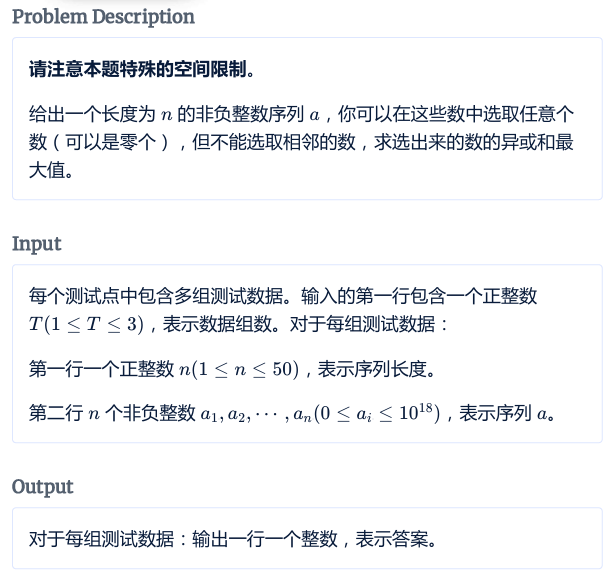
\includegraphics[width=0.78\linewidth]{assets/e050_image-4.png}\end{center}


\begin{codeline}
const int N = 55;
int n;

inline long long highBit(long long num) {
    if(!num) {
        return 0ll;
    } else {
        return num & (1ll << (64 - __builtin_clzll(num) - 1));
    }
}

class HamelBasis {
public:
    int maxn;
    int cnt;
    vector<long long> vec;

    /*
     * 清空线性基，预留_n个向量
     */
    void init(int _n) {
        maxn = _n;
        cnt = 0;
        vec.clear();
        vec.resize(_n);
    }

    /*
     * 插入num，返回插入位置；相关向量返回-1
     */
    int insert(long long num) {
        for(int i = maxn - 1; ~i && num; i--) {
            if(num & (1ll << i)) {
                if(!vec[i]) {
                    vec[i] = num;
                    return i;
                } else {
                    num ^= vec[i];
                }
            }
        }
        return -1;
    }
    /*
     * 撤销idx处的向量插入
     */
\end{codeline}
\vspace{-0.9\baselineskip}
\begin{codeline}[firstnumber=47]
    void pop(int idx) {
        vec[idx] = 0;
    }

    /*
     * 求num与线性基能表示的数异或后的最大值
     */
    long long getMax(long long num = 0) {
        long long ans = num;
        for(int i = maxn - 1; ~i; i--) {
            if(!(ans & (1ll << i)) && vec[i]) {
                ans ^= vec[i];
            }
        }
        return ans;
    }
};

HamelBasis basis;

long long a[N];
long long ans;

void dfs(int k) {
    if(k >= n) {
        ans = max(ans, basis.getMax());
        return;
    }
    int idx = basis.insert(a[k]);
    dfs(k + 2);
    dfs(k + 3);
    if(idx >= 0) {
        basis.pop(idx);
    }
}

int main() {
    ios::sync_with_stdio(false);
    cin.tie(nullptr);
    int T;
    cin >> T;
    while(T--) {
        cin >> n;
        for(int i = 0; i < n; i++) {
            cin >> a[i];
        }
\end{codeline}
\vspace{-0.9\baselineskip}
\begin{codeline}[firstnumber=93]
        ans = 0;
        basis.init(60);
        dfs(0);
        dfs(1);
        cout << (ans) << '\n';
    }
}
\end{codeline}
\begin{warnbox}
插入按最高位消元；查询最大值从高位贪心。
\end{warnbox}

\section{线性方程组}
\entrymeta{$O(n^3)$}
\subsection{P2455 {[}SDOI2006{]} 线性方程组}\label{p2455-sdoi2006-ux7ebfux6027ux65b9ux7a0bux7ec4}


\begin{codeline}
class LinearSystem {
public:
    static const int N = 55;
    static constexpr double EPS = 1e-9;

    int n = 0;
    double a[N][N + 1];

    /*
     * 初始化 n 元方程组，系数矩阵清零
     */
    void init(int n_) {
        n = n_;
        for(int i = 0; i < n; i++) {
            for(int j = 0; j <= n; j++) {
                a[i][j] = 0;
            }
        }
    }

    /*
     * 高斯-约当消元。返回 -1 无解、0 无穷多解、1 唯一解；
     * 唯一解时 a[i][n] 即 x_{i+1}
     */
    int solve() {
        int rank = 0;
        for(int col = 0; col < n && rank < n; col++) {
            int pivot = -1;
            for(int r = rank; r < n; r++) {
                if(abs(a[r][col]) > EPS) {
                    pivot = r;
                    break;
                }
            }
            if(pivot == -1) {
                continue;
            }
            for(int j = 0; j <= n; j++) {
                swap(a[rank][j], a[pivot][j]);
            }
            double k = a[rank][col];
            for(int j = col; j <= n; j++) {
                a[rank][j] /= k;
            }
            for(int r = 0; r < n; r++) {
                if(r == rank || abs(a[r][col]) <= EPS) {
\end{codeline}
\vspace{-0.9\baselineskip}
\begin{codeline}[firstnumber=47]
                    continue;
                }
                double f = a[r][col];
                for(int j = col; j <= n; j++) {
                    a[r][j] -= f * a[rank][j];
                }
            }
            rank++;
        }

        for(int i = rank; i < n; i++) {
            if(abs(a[i][n]) > EPS) {
                return -1;
            }
        }
        return rank < n ? 0 : 1;
    }
};

int main() {
    ios::sync_with_stdio(false);
    cin.tie(nullptr);
    int n;
    cin >> n;
    LinearSystem ls;
    ls.init(n);
    for(int i = 0; i < n; i++) {
        for(int j = 0; j <= n; j++) {
            cin >> ls.a[i][j];
        }
    }

    int res = ls.solve();
    if(res == -1) {
        cout << -1 << '\n';
        return 0;
    }
    if(res == 0) {
        cout << 0 << '\n';
        return 0;
    }
    for(int i = 0; i < n; i++) {
        double x = abs(ls.a[i][n]) < LinearSystem::EPS ? 0.0 : ls.a[i][n];
        cout << "x" << (i + 1) << "=" << fixed << setprecision(2) << x << '\n';
    }
    return 0;
\end{codeline}
\vspace{-0.9\baselineskip}
\begin{codeline}[firstnumber=93]
}
\end{codeline}
\begin{warnbox}
返回 -1 无解、0 无穷多解、1 唯一解；唯一解在 \texttt{a[i][n]}。
\end{warnbox}

\section{拉格朗日插值}
\entrymeta{$O(n^2)$ 预处理}
调用前提：先 init，x/y 长度一致；moder 为质数，x 模意义互异。


\begin{codeline}
// moder 为质数，x 在模 moder 下两两不同；O(n^2 log moder)。
class Interpolation {
public:
    int64 moder = 998244353;
    int64 norm(int128 a) const {
        return (a % moder + moder) % moder;
    }

    vector<int64> x, y;
    /*
     * 分配n+1个插值点，调用处填充x、y
     */
    void init(int n) {
        x.assign(n + 1, 0);
        y.assign(n + 1, 0);
    }
    /*
     * 根据插值点求t处的函数值，x在模moder下须两两不同
     */
    int64 operator()(int64 t) const {
        int64 ans = 0;
        for(int i = 0; i < int(x.size()); i++) {
            int64 p = norm(y[i]);
            for(int j = 0; j < int(x.size()); j++) {
                if(i != j) {
                    int64 div = norm(int128(x[i]) - x[j]);

                    p = norm(int128(p) * norm(int128(t) - x[j]));
                    p = norm(int128(p) * quickPow(div, moder - 2, moder));
                }
            }
            ans = norm(int128(ans) + p);
        }
        return ans;
    }
};
\end{codeline}
\begin{warnbox}
分母用费马小定理求逆；需要模数为素数。
\end{warnbox}


\chapter{组合}

\section{容斥原理}
\entrymeta{$O(4s + 2^4 n)$}
\subsection{P1450 {[}HAOI2008{]} 硬币购物}\label{p1450-haoi2008-ux786cux5e01ux8d2dux7269}


\begin{codeline}
const long long N = 100005;
long long c[5];
long long n;
long long d[5];
long long s;
long long dp[N];
int main() {
    ios::sync_with_stdio(false);
    cin.tie(nullptr);
    cin >> c[0] >> c[1] >> c[2] >> c[3] >> n;
    for(long long T = 1; T <= n; T++) {
        cin >> d[0] >> d[1] >> d[2] >> d[3] >> s;

        for(long long i = 0; i <= s; i++) {
            dp[i] = 0;
        }

        dp[0] = 1;
        for(long long i = 0; i < 4; i++) {
            for(long long j = c[i]; j <= s; j++) {
                dp[j] += dp[j - c[i]];
            }
        }

        long long ans = 0;
        for(long long i = 0; i < 1 << 4; i++) {
            long long k = s;
            for(long long j = 0; j < 4; j++) {
                if((i >> j) & 1) {
                    k -= c[j] * (d[j] + 1);
                }
            }
            if(k >= 0) {
                if(__builtin_popcountll(i) & 1) {
                    ans -= dp[k];
                } else {
                    ans += dp[k];
                }
            }
        }
        cout << (ans) << '\n';
    }
}
\end{codeline}
\begin{warnbox}
每组询问重跑背包会超时；先读入所有询问取 maxS 预处理。
\end{warnbox}

\section{约瑟夫环问题}
\entrymeta{$O(n)$ 或 $O(k\log n)$}
\subsection{问题描述}\label{ux95eeux9898ux63cfux8ff0}

\begin{quote}
n 个人标号 \(0,1,\cdots, n-1\)。逆时针站一圈，从 \(0\) 号开始，每一次从当前的人逆时针数 \(k\) 个，然后让这个人出局。问最后剩下的人是谁。
\end{quote}

\subsection{过程}\label{ux8fc7ux7a0b}

\subsubsection{朴素算法}\label{ux6734ux7d20ux7b97ux6cd5}

最朴素的算法莫过于直接枚举。用一个环形链表枚举删除的过程，重复 \(n-1\) 次得到答案。复杂度 \(\Theta (n^2)\)。

\subsubsection{简单优化}\label{ux7b80ux5355ux4f18ux5316}

寻找下一个人的过程可以用线段树优化。具体地，开一个 \(0,1,\cdots, n-1\) 的线段树，然后记录区间内剩下的人的个数。寻找当前的人的位置以及之后的第 \(k\) 个人可以在线段树上二分做。

\subsubsection{线性算法}\label{ux7ebfux6027ux7b97ux6cd5}

设 \(J_{n,k}\) 表示规模分别为 \(n,k\) 的约瑟夫问题的答案。我们有如下递归式

\[
J_{n,k}=(J_{n-1,k}+k)\bmod n
\]

这个也很好推。你从 \(0\) 开始数 \(k\) 个，让第 \(k-1\) 个人出局后剩下 \(n-1\) 个人，你计算出在 \(n-1\) 个人中选的答案后，再加一个相对位移 \(k\) 得到真正的答案。这个算法的复杂度显然是 \(\Theta (n)\) 的。


\begin{codeline}
/*
 * 返回每次数到k出局后的幸存者编号，从0开始
 */
int josephus(int n, int k) {
    int res = 0;
    for(int i = 1; i <= n; ++i) {
        res = (res + k) % i;
    }
    return res;
}
\end{codeline}


\subsubsection{对数算法}\label{ux5bf9ux6570ux7b97ux6cd5}

对于 \(k\) 较小 \(n\) 较大的情况，本题还有一种复杂度为 \(\Theta (k\log n)\) 的算法。

考虑到我们每次走 \(k\) 个删一个，那么在一圈以内我们可以删掉 \(\left\lfloor\frac{n}{k}\right\rfloor\) 个，然后剩下了 \(n-\left\lfloor\frac{n}{k}\right\rfloor\) 个人。这时我们在第 \(\left\lfloor\frac{n}{k}\right\rfloor\cdot k\) 个人的位置上。而你发现它等于 \(n-n\bmod k\)。于是我们继续递归处理，算完后还原它的相对位置。还原相对位置的依据是：每次做一次删除都会把数到的第 \(k\) 个人删除，他们的编号被之后的人逐个继承，也即用 \(n-\left\lfloor\frac{n}{k}\right\rfloor\) 人环算时每 \(k\) 个人即有 \(1\) 个人的位置失算，因此在得数小于 \(0\) 时，用还没有被删去 \(k\) 倍数编号的 \(n\) 人环的 的 \(n\) 求模，在得数大于等于 \(0\) 时，即可以直接乘 \(\frac{k}{k-1}\), 于是得到如下的算法：


\begin{codeline}
/*
 * 返回每次数到k出局后的幸存者编号，从0开始
 */
int josephus(int n, int k) {
    if(n == 1) {
        return 0;
    }
    if(k == 1) {
        return n - 1;
    }
    if(k > n) {
        return (josephus(n - 1, k) + k) % n; // 线性算法
    }
    int res = josephus(n - n / k, k);
    res -= n % k;
    if(res < 0) {
        res += n; // mod n
    } else {
        res += res / (k - 1); // 还原位置
    }
    return res;
}
\end{codeline}


可以证明这个算法的复杂度是 \(\Theta (k\log n)\) 的。我们设这个过程的递归次数是 \(x\)，那么每一次问题规模会大致变成 \(\displaystyle n\left(1-\frac{1}{k}\right)\)，于是得到

\[
n\left(1-\frac{1}{k}\right)^x=1
\]

解这个方程得到

\[
x=-\frac{\ln n}{\ln\left(1-\frac{1}{k}\right)}
\]

\begin{warnbox}
两个版本二选一；注意 k ≥ 1、n ≥ 1。
\end{warnbox}

\section{康托展开}
\entrymeta{$O(n\log n)$}
\subsection{P5367 【模板】康托展开}\label{p5367-ux6a21ux677fux5eb7ux6258ux5c55ux5f00}










\begin{codeline}
class Cantor {
    static constexpr int64 MODER = 998244353;

public:
    // a[1..n] 是 1..n 的排列，返回从 1 开始的排名。
    int64 rank(const vector<int>& a) const {
        int n = int(a.size()) - 1;
        vector<int> arr(n + 1);
        vector<int64> fac(n + 1, 1);
        for(int i = 1; i <= n; i++) {
            arr[i] = i & -i;
            fac[i] = fac[i - 1] * i % MODER;
        }
        int64 ans = 1;
        for(int i = 1; i <= n; i++) {
            int cnt = 0;
            for(int j = a[i] - 1; j; j -= j & -j) {
                cnt += arr[j];
            }
            ans = (ans + cnt * fac[n - i]) % MODER;
            for(int j = a[i]; j <= n; j += j & -j) {
                arr[j]--;
            }
        }
        return ans;
    }
};
\end{codeline}
\begin{warnbox}
配合树状数组求排名；阶乘取模。
\end{warnbox}


\chapter{计算几何}

\section{扫描线}
\entrymeta{$O(n\log n)$}
\subsection{P5490 【模板】扫描线 \& 矩形面积并}\label{p5490-ux6a21ux677fux626bux63cfux7ebf-ux77e9ux5f62ux9762ux79efux5e76}


\begin{codeline}
const int N = 100005;
const int M = 1000000007;
int n;

class Data {
public:
    int cnt;

    Data operator+(const Data& other) const {
        return {cnt + other.cnt};
    }
};

class Tag {
public:
    int add;

    Tag operator+(const Tag& other) const {
        return {add + other.add};
    }

    /*
     * 标记持久化：add 是累积覆盖次数，> 0 时整段都被覆盖
     */
    Data apply(const Data& d, int l, int r) const {
        if(add > 0) {
            return {r - l + 1};
        }
        return d;
    }
};

class Line {
public:
    int x1, x2;
    int y;
    bool upper;

    bool operator<(const Line& other) const {
        return y < other.y;
    }
};

Line line[N * 2];

/*
\end{codeline}
\vspace{-0.9\baselineskip}
\begin{codeline}[firstnumber=47]
 * 注意：这里用的是标记持久化线段树，标记不下传，不是普通的懒惰标记线段树。
 * Tag::apply 接收的是累积后的标记；原理见 数据结构/线段树/标记持久化线段树.md。
 */
SegmentTree<Data, Tag> sgt;

int main() {
    ios::sync_with_stdio(false);
    cin.tie(nullptr);
    cin >> n;
    sgt.init(0, M, 32 * n);
    int x1, x2, y1, y2;

    for(int i = 0; i < n; i++) {
        cin >> x1 >> y1 >> x2 >> y2;
        line[i * 2] = {x1, x2 - 1, y1, false};
        line[i * 2 + 1] = {x1, x2 - 1, y2, true};
    }

    sort(line, line + n * 2);

    long long w = 0;
    long long ly = 0;
    long long s = 0;
    for(int i = 0; i < n * 2; i++) {
        s += w * (line[i].y - ly);
        if(line[i].upper) {
            sgt.mod(line[i].x1, line[i].x2, {-1});
        } else {
            sgt.mod(line[i].x1, line[i].x2, {1});
        }
        w = sgt.query(0, M).cnt;
        ly = line[i].y;
    }
    cout << (s) << '\n';
}
\end{codeline}
\begin{warnbox}
依赖标记持久化线段树：覆盖次数 > 0 返回区间全长，否则合并儿子。
\end{warnbox}

